\documentclass{tufte-handout}

\title{On ultimate; O5: left handler}
\author[James Reynolds]{James Reynolds}

%\date{28 March 2010} % without \date command, current date is supplied

%\geometry{showframe} % display margins for debugging page layout

\usepackage{graphicx} % allow embedded images
  \setkeys{Gin}{width=\linewidth,totalheight=\textheight,keepaspectratio}
  \graphicspath{{graphics/}} % set of paths to search for images
\usepackage{amsmath}  % extended mathematics
\usepackage{booktabs} % book-quality tables
\usepackage{units}    % non-stacked fractions and better unit spacing
\usepackage{multicol} % multiple column layout facilities
\usepackage{lipsum}   % filler text
\usepackage{fancyvrb} % extended verbatim environments
  \fvset{fontsize=\normalsize}% default font size for fancy-verbatim environments

% Standardize command font styles and environments
\newcommand{\doccmd}[1]{\texttt{\textbackslash#1}}% command name -- adds backslash automatically
\newcommand{\docopt}[1]{\ensuremath{\langle}\textrm{\textit{#1}}\ensuremath{\rangle}}% optional command argument
\newcommand{\docarg}[1]{\textrm{\textit{#1}}}% (required) command argument
\newcommand{\docenv}[1]{\textsf{#1}}% environment name
\newcommand{\docpkg}[1]{\texttt{#1}}% package name
\newcommand{\doccls}[1]{\texttt{#1}}% document class name
\newcommand{\docclsopt}[1]{\texttt{#1}}% document class option name
\newenvironment{docspec}{\begin{quote}\noindent}{\end{quote}}% command specification environment

\begin{document}

\maketitle% this prints the handout title, author, and date
%\printclassoptions
This is 
a two-pager 
about
playing 
on offence 
as the left handler,  
referred to here 
as position O5\footnote{This
is part of a series, 
available at
\url{https://github.com/James-Reynolds/Ultimate-strategy-and-tactics}}. 
The handler positions (O5-7) 
are generally interchangeable, 
and you may find yourself 
playing on the left (O5), 
in the centre (O6), 
and on the right (O7) 
within 
a single possession.  
Additionally, 
handling is a 
group, 
rather than individual,
activity.
It is not just where you throw to 
that matters; 
where you stand, 
when and where you move, 
and what you do 
when you don't have the disc is 
important too!   
This document 
focuses on 
handling 
on the left 
side of the field
(as you look downfield), 
but you might also 
want to read the two-pagers about 
O6 
and O7 
for thoughts on 
handling elsewhere. 

\section{Receiving the pull} 
\label{sec:vertical}
\begin{marginfigure}%
  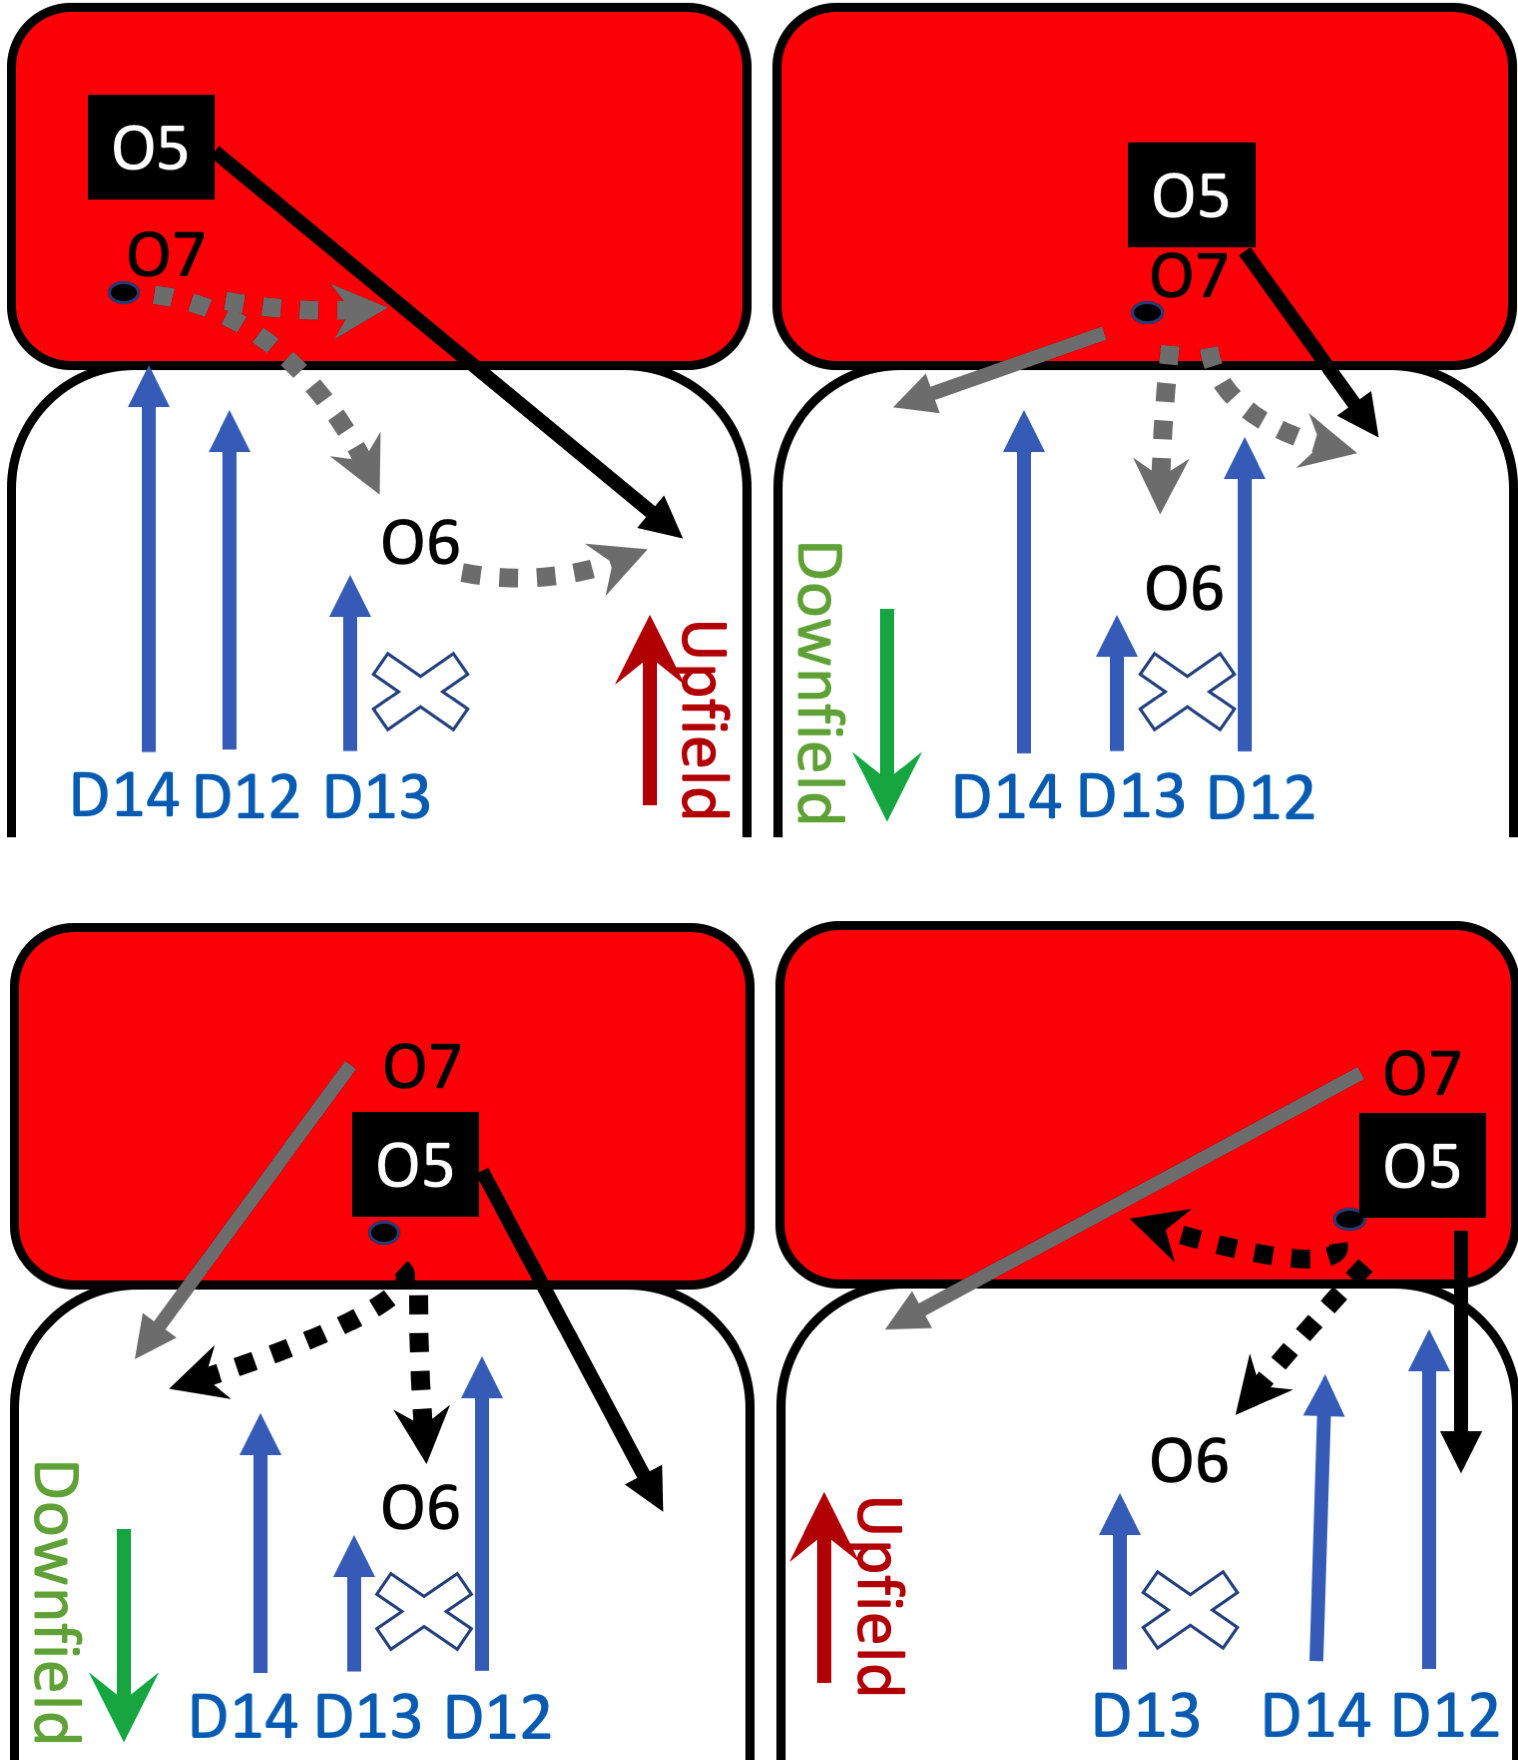
\includegraphics[width=\linewidth]{O5-pull}
  \caption{Potential formations for receiving a pull: 
  O7 (top-left, top-right), and O5 (bottom-left, bottom-right)}
  \label{fig:O5-pull}
\end{marginfigure}
Objectives 
when receiving the pull,
in order of importance, 
would seem to be:
(1) do not turn it over\footnote{
Trying to catch the pull 
risks dropping it.  
Letting it 
touch the ground first 
costs time. 
Are you really in all 
that much of a hurry 
to make the first pass?};
(2) defend against a roller\footnote{
If it rolls out the 
back of the endzone, 
you get to put it in play 
from the front of the endzone, 
unless someone on your team 
has touched it before it went out 
(in which case 
it is played from 
the back of the endzone, 
which is often very hard).
Again, are you really in all 
that much of a hurry 
to make the first pass?}; 
(3) execute a set play off the pull 
(if there is one); 
(4) improve the position of the disc 
(e.g. move it to the centre of the field) 
and (5) set up a handler in a good spot 
to throw the next pass; 
(6) make territory by moving the disc downfield; and 
(7) give the cutters (O1-4) time to get downfield 
and into the called formation. 
All of this 
needs to be 
balanced against 
the risk of giving up 
a quick turnover\footnote{Often via 
a run-through 
interception.  
Perhaps this is because 
the defenders running upfield
tend to have some speed up, 
while the handlers are often 
static.}.

Figure \ref{fig:O5-pull}
shows four pull receptions. 
In the top-left, 
O7 is shown 
taking possession. 
You (O5) 
are shown 
providing a 
second line of defence 
against a particularly 
good roller-pull 
(Objective 2)\footnote{
Another advantage of 
being behind O7 
as they catch the pull 
is that you will be able to 
see them AND everyone else. 
Hence, you can tell them how soon 
the defence will arrive, 
whether it is person-match 
or zone, etc.}.  
From there, you might 
proceed back across to the 
left side (looking downfield) 
of the field 
(black arrow). 
O7 has the option of 
centring (dashed grey lines) 
the disc to you 
(Objective 4) 
or centring 
and throwing downfield 
to O6 
(Objectives 4 and 5)\footnote{
A further dashed grey line 
indicates how O6 
might then pass to you, 
putting you in a good position 
to throw down the break side 
(Objective 5).}. 

The other three panels 
in Figure \ref{fig:O5-pull} 
show variations 
on the same theme. 
But, there are endless 
possibilities depending 
on what sort of pull is thrown. 
Ideally, 
your opposition throws it out  
(and then you can call a brick) 
or short, giving you a good position 
and time for the cutters to set up  
(Objectives 4, 6 and 7). 

\section{A few higher risk throws, or many lower risk throws? }\label{sec:risk}
Aims 
on offence are: 
(1) score a goal; and
(2) do not let 
your opposition 
score, with 
sub-goals
(2a) do not turn the disc over, 
and 
(2b) if there is a turnover, 
get one back. 
The trade-offs 
are likely 
subjective 
and variable\footnote{
For example, on a 
downwind point 
with poor weather 
and a lack of players
on your team who are good 
at throwing in the wind, 
you might ignore (2a) 
and instead play huck-(1)-and-zone (2b). 
In contrast, 
games in conditions favouring 
offence might 
be won by the team 
with the least number of
throw aways (2a!).}.
However, 
the risk of a turnover 
likely increases with the: 
(A) number of throws; 
(B) risk of turnover for each throw attempted; and 
(C) quality of the defence, and 
(D) the stall count.  
Hence, 
if your team 
is good at disc retention\footnote{
Or at least 
better 
at disc retention 
than your opposition,  
as least turnovers 
(typically) wins!}.
you might seek to 
only take 
high percentage options, 
assuming that you 
will eventually 
get a low-risk opportunity 
to score.  
Alternatively, 
in the face 
of a high-quality 
defence, 
your team might be willing to 
send a low-percentage huck early on, 
assuming that you are 
probably going to turn it over 
within a small number of passes 
anyway so you might as well 
have a shot at scoring immediately\footnote{
There are further levels to consider. 
For example, sending some 
hucks early on in the game, 
even if unsuccessful, 
might spook the defenders. 
This might then make it 
easier to throw to upfield cuts 
during the rest of the game.}.  

An important factor 
in this equation 
is whether your team
is typically able to 
retain possession using a dump. 
It appears that 
much of the challenge in dumping 
is positioning, 
rather than the throws themselves. 
As left-handler, 
you will
be on the break side 
when there is 
a forehand force 
(for right handers).  

TRANSITION INTO DUMP DISCUSSION










\section{Beating person-match defence with a vertical stack}\label{sec:vertical}

\begin{marginfigure}%
  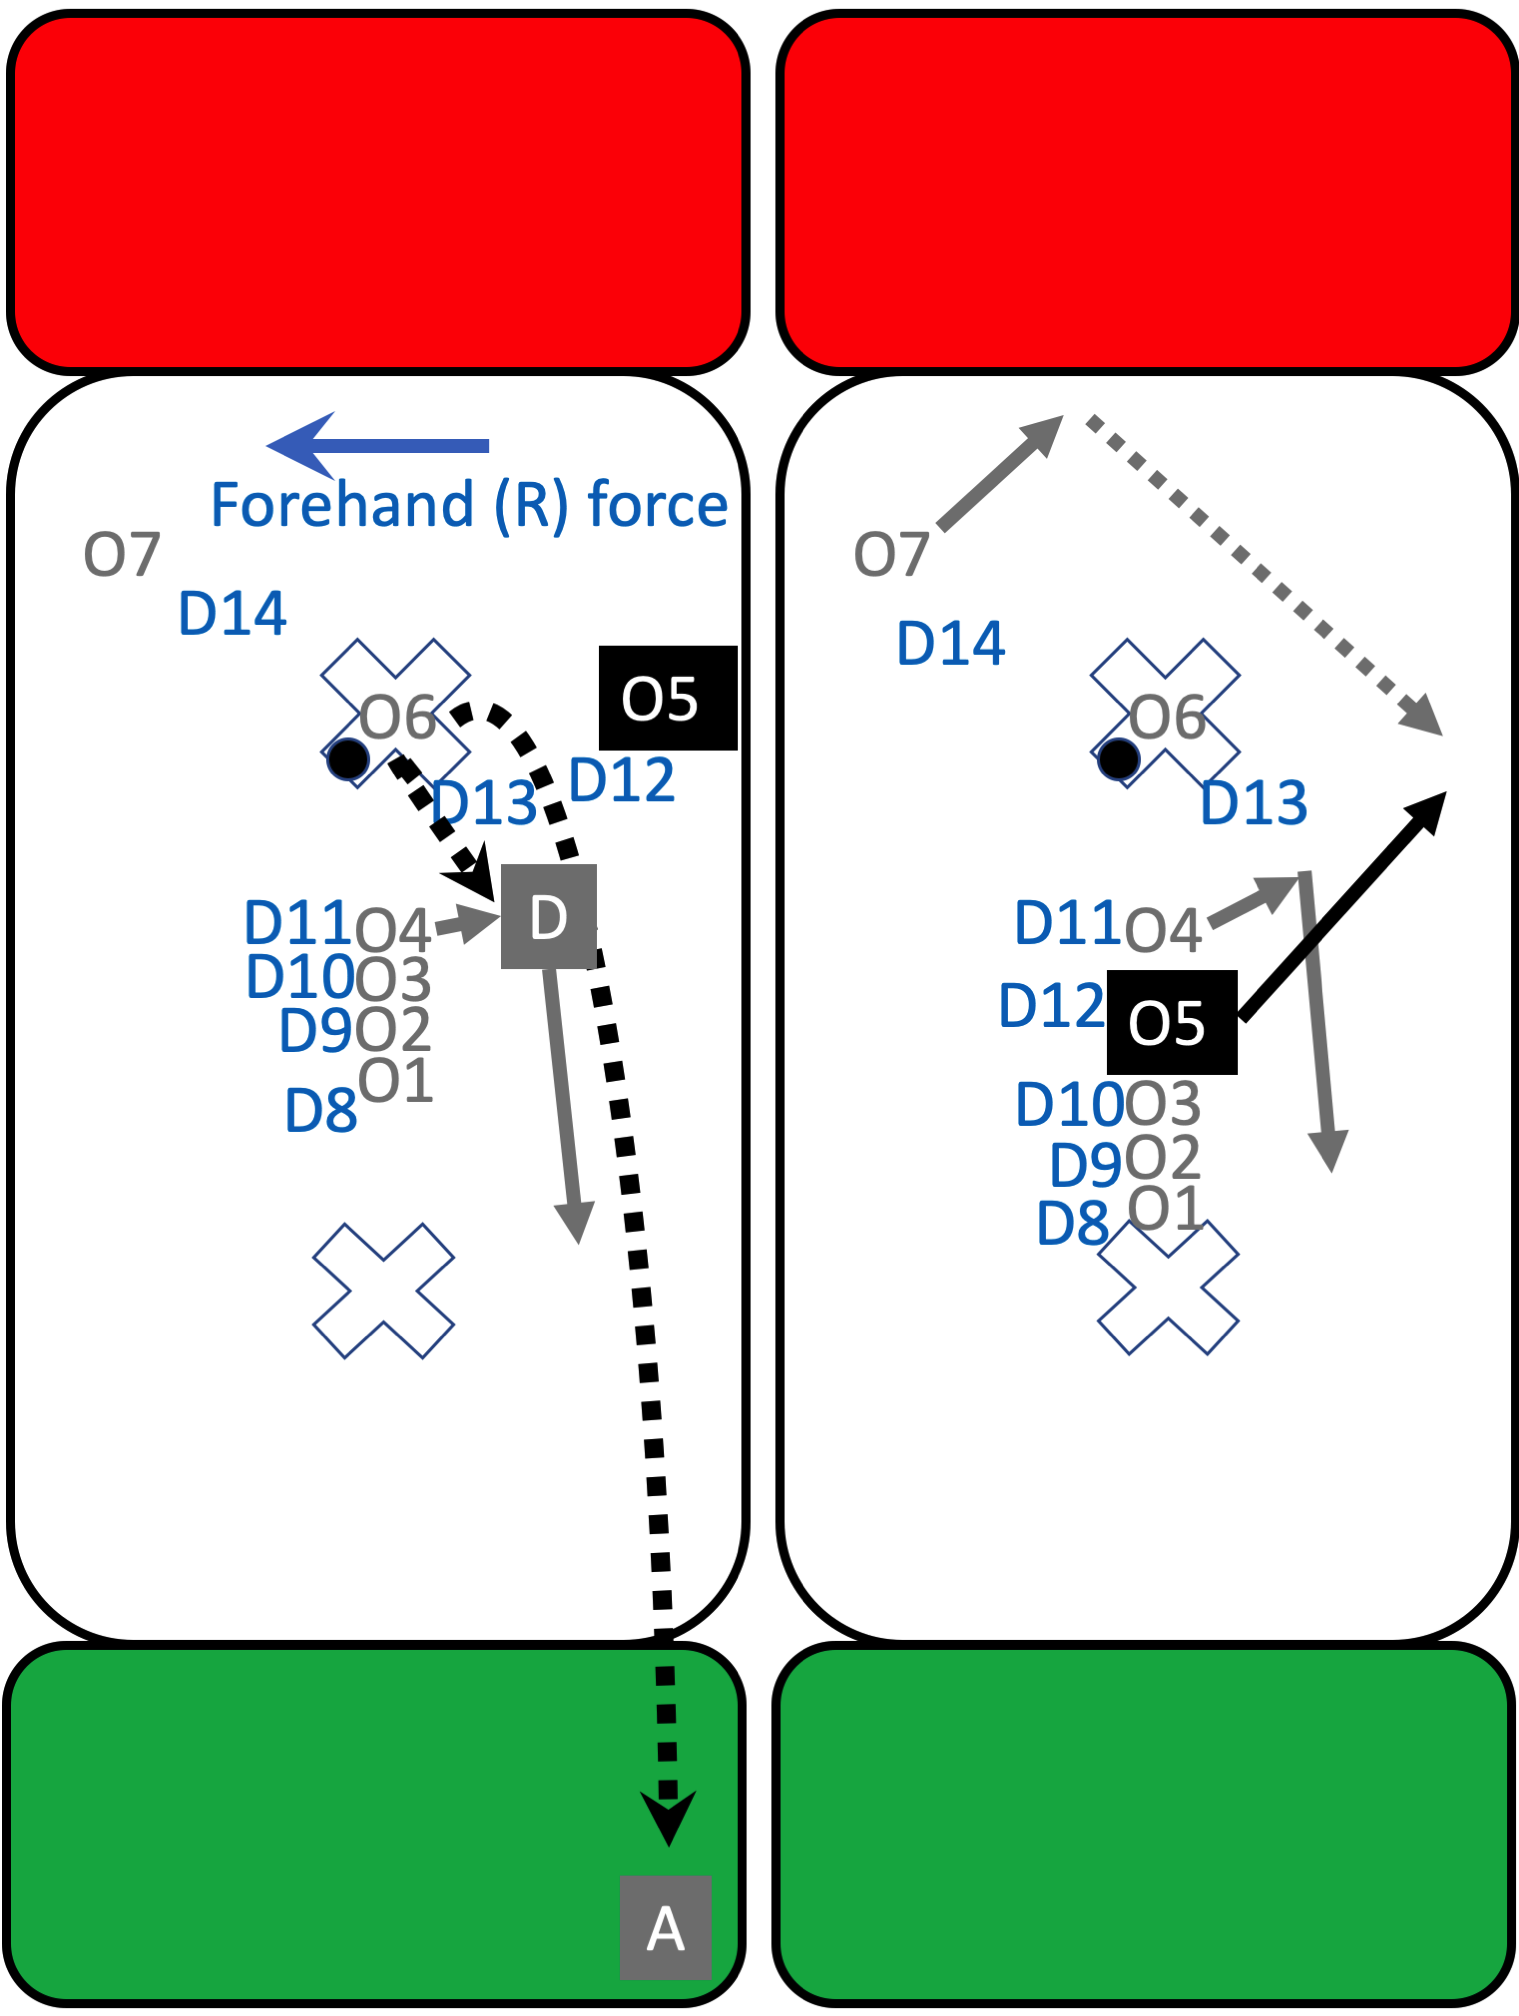
\includegraphics[width=\linewidth]{O5-vertical}
  \caption{Vertical stack: 
  starting position (left),
  D11 poaching deep (top-right) 
  and disc moved to C means D11 
  covers O5 (bottom-right)}
  \label{fig:O5-vertical}
\end{marginfigure}

Figure \ref{fig:O5-vertical} (left) shows 
your team: 
using 
a vertical stack formation; 
having called a brick; and
facing a 
forehand force with 
person-match defence\footnote{
Vertical works
against other person-match defences, 
but might need 
adjustment e.g. 
(1) backhand force,
mirror everything;
(2) straight up force, 
maybe give the handlers 
time to move the disc around, 
and go out to the sidelines
when you do cut; etc.}. 
You (O5) 
are shown 
at the front 
of the stack.
D11 
is likely to set up, 
as shown, 
to defend the open side. 
O6 might
therefore be 
able to 
throw a break-force 
you going to D\footnote{
You may
be able to stand still, 
simply wait for O6 
to throw, 
and then run onto 
it at D.}.
If you do not 
receive the disc 
at D, 
you might then 
cut downfield 
on the break side 
of the field, 
heading towards 
A\footnote{
Watch out that you 
do not cause a pick 
between D11, 
D10 and O3.}.  

The third, 
solid black arrow
shown in 
Figure \ref{fig:O5-vertical} (left) 
indicates you 
returning to 
the rear of the stack, 
or you might continue 
and cut to C. 
However, the dashed, 
red, 
horizontal line 
indicates the limit 
of how far you 
would go downfield\footnote{
The position of 
this line 
varies with movement 
of the disc and the distance 
that the person with the disc 
can (or is likely to) throw.
The dashed, 
yellow line, 
similarly indicates 
approximately the
limit of how far you 
would go upfield.  
Any further and
you are crowding the handlers, 
and your defender 
might be able to interfere 
with the dump}. 
Figure \ref{fig:O5-vertical} (top-right) shows 
what might happen 
if you go downfield of
the dashed red line 
prior to the disc being thrown. 
Because the disc travels slowly 
through the air, 
D11 will no longer has to stay as close to you 
to prevent or intercept a throw 
(to you and/or A)
D11 is therefore able to play 
further upfield 
so as to 
cover you if you 
cut back towards 
the disc. 
They might also 
poach, so as to 
potentially intercept
or prevent 
downfield throws 
to O1-3\footnote{
Note how Figure \ref{fig:O5-vertical} (top-right)  
shows D8-10 
having changed their 
positioning 
to cover O1-3
almost exclusively upfield, 
preventing the under cut.  
This is possible because you (O5) 
are so deep, 
that D8-10 may be 
able to rely on 
D11 intercepting 
or preventing any deep throws 
to their direct opponents.}. 

Figure \ref{fig:O5-vertical} (bottom-right)  
provides an example 
of a similar situation, but 
where the disc has moved 
in the meantime to O1, 
who cut to C.  
The dashed,
red,
horizontal line 
is shown 
further downfield in 
Figure \ref{fig:O5-vertical} (bottom-right), 
reflecting that if O1 
throws the disc to 
A it will arrive 
more quickly than before, 
when O6 had it further upfield. 
Hence, D11 will likely 
have to play tighter defence 
on you (O5), 
meaning that O2 and O3 
will be able to cut deep to B.

As primary long, 
your role is 
typically to provide 
a target for a scoring throw 
into the endzone, or 
otherwise gain a lot of 
territory. If you do get the disc,
you might be able to immediately
pass to one of the other cutters 
(O1-3). 
However, 
you are also cutter, 
so the most 
important things to do are:
to make sure your team 
retains possession of the disc.
Hence, 
if no (safe) pass downfield 
is immediately available, 
it is probably time to engage 
one of the handlers (O5-7), 
throw a dump, 
and get downfield again 
to do some more cutting.  
The handlers can take care
of the throwing, 
but your team likely 
needs you to be a target, 
which the handlers are likely 
too far upfield to provide.


\subsection{Beating person-match defence with feldrunner}
\label{sec:feld}
%\begin{marginfigure}%
 % \includegraphics[width=\linewidth]{O5-horizontal}
 % \caption{Feld (left) \& ho-ro (right)}
 % \label{fig:O5-horizontal}
%\end{marginfigure}
Figure \ref{fig:O5-horizontal} (left) 
shows a feldrunner formation, 
O1 as the focus, and 
O2 and O3 
in the endzone. 
You are one 
of the four handlers. 
The idea of feldrunner 
is to pass to 
the isolated
focus (O1). 
They then either pass to 
O2 or O3, 
or dump to the handlers
and reset. 
Typically you, 
O5, 
O6 
and O7 
try to stay out of the way 
when you don't have the disc. 

If you do have the disc 
you will be trying
to throw to O1. 
If D8 
is looking at O1 
you can throw 
into the space behind, 
allowing O1 to run onto it. 
Alternatively, if 
D8 looks at you, 
O1 can likely cut
and get clear enough 
for you to pass to them. 

\subsection{Beating person-match defence with a horizontal stack}\label{sec:horizontall}
Horizontal stack 
typically involves cutting
upfield and downfield (black arrows)
within your quarter of the field\footnote{
Other cuts
can work, 
but might need
communication,
e.g. diamond cuts 
involve trading places 
with O3.}
as shown in 
Figure \ref{fig:O5-horizontal}(right).
O6 
can potentially 
throw to you 
in the endzone 
or at C\footnote{
Black arrows
show how a back-under cut 
opens space 
for the throw 
to C.}. 

\section{Beating zone defence}\label{sec:zone}
%\begin{marginfigure}%
 % \includegraphics[width=\linewidth]{O5-zone331}
 % \caption{formations against 331 zone}
 % \label{fig:O5-zone331}
%\end{marginfigure}
Vertical stack 
probably won't work 
against zone.. 
Instead, your 
team needs to 
spread out. 
Three ways to beat a zone are:
(1) over;
(2) round; or
(3) through. 
Figure \ref{fig:O5-zone331}
(top left)
shows this 
against a 
3-3-1 zone, 
with a throw 
direct 
from O6 
\smallcaps{over} to you\footnote{
This may be a 
blade or
hammer, 
to get it 
to you
as quickly as possible.
So it may help to 
stand still 
and look at O6.}.
Otherwise, 
O6 might throw
over or through (to O2 or O3), 
or round (to O5 or O7)\footnote{
You, 
O3, 
and O7
might then split
D8 and D11 
to make ground 
before the cup 
(D12-14) catch up. 
Once they do, 
dump to O6 
so all 7 of your players
are involved again.}. 

If the defence 
continues to play zone 
once the disc 
gets close to the endzone, 
you (O5) 
and the other wing (O1) 
can \smallcaps{go and stand 
on the back corners}
(Figure \ref{fig:O5-zone331} (bottom left)\footnote{ 
The defence 
will either  
leave you open,
or cover you
at the corner
(D8)
making more space 
for O2, 
O3 and
O5-7 
at the front of the endzone.}.
Figure \ref{fig:O5-zone331} (bottom right) shows 
how the further 
you are from the back corner 
the more D8  
can cover both you
AND others, 
and the harder 
it is to throw direct to you.
D11 might even be able to
guard O7 closely, if 
you end up close enough to 
O2 and O3. 
This applies also when 
not close to the endzone 
(top right).
If you crowd forward,
D8 only has to cover O1, 
and D9 and D11 
can push upfield.


\section{Beating clam defence}\label{sec:zone}
Clam mixes person-match 
and zone defence styles, 
with defenders 
switching frequently.
%\footnote{
%For example, 
%in Figure \ref{fig:O5-vertical}(left) 
%D8 
%might cover 
%O1 deep, 
%switching later 
%(with D9 or D11
%to cover O5's cut deep,
%rather than following O1 
%upfield to C.}. 
You might
coordinate 
with others  
to overload 
a defender, 
or spread out 
and give the handlers 
space 
and targets deep. 

\newthought{...and finally} 
this is just a two pager; 
there are many more 
offensive strategies 
and tactics\footnote{
Try U-stack: two side stacks, 
one on each side, and
three handlers back.  
Leaving space in the middle of the field. }
Remember, 
defence wins games, 
offence loses them\footnote{
Because the team with the least turnovers 
usually wins.};.
and it's better to get it back 
with another turnover\footnote{
i.e. if you offence fails, its time to play defence, even though you're the O team :)}
than receiving another pull!

\end{document}
